\chapter{Actuator Disc Method}

\section{Assumptions}

Following assumptions are made for the purpose of modeling helicopter rotor aerodynamics:
\begin{itemize}
  \item[---] forces and moments generated by the rotor are considered to be quasi-steady,
  \item[---] rotor lift force is a linear function of blade incidence angle and drag force is a quadratic function of lift, \cite{Padfield2007}
  \item[---] rotor blades have 3 degrees of freedom movement,
  \item[---] inflow is uniformly distributed over rotor disc, \cite{Padfield2007}
  \item[---] reversed flow effects are ignored,
  \item[---] airflow is considered to be quasi-steady and incompressible,
  \item[---] thrust is considered to be parallel to the z-axis of the Control Axis System and magnitude of the thrust is considered to be magnitude of the resulting rotor force. \cite{GessowMyers1985}
\end{itemize}

\section{Momentum Theory}

\subsection{Momentum Theory for Axial Flight}

Mass flow through the rotor disc, momentum change and change in kinetic energy are given by the following formulas. \cite{Padfield2007}
\begin{align}
  \label{eq-aero-mass-flow}
  \dot m
  &=
  \rho A_1 V_C = \rho A_R \left( V_C + V_i \right)
  =
  \rho A_{i \infty} \left( V_C + V_{i \infty}  \right) \\
  \label{eq-aero-thrust-1}
  T
  &=
  \dot m \left( V_C + V_{i \infty} \right)
  -
  \dot m V_C = \dot m V_{ i \infty } \\
  T \left( V_C + V_{ i \infty } \right)
  &=
  \frac{1}{2} \dot m \left( V_C + V_{ i \infty } \right)^2
  -
  \frac{1}{2} \dot m V_C^2
  =
  \frac{1}{2} \dot m \left( 2V_C V_{ i \infty } + V_{ i \infty }^2 \right)
\end{align}

Where:
\begin{description}[align=right,labelwidth=3cm]
  \item [$A_1 = \pi R_1^2$] [m\textsuperscript{2}] control volume section area
  \item [$A_R = \pi R^2$] [m\textsuperscript{2}] rotor disc area
  \item [$A_{\infty} = \pi R_{\infty}^2$] [m\textsuperscript{2}] far wake slipstream section area
  \item [$\dot m$] [kg/s] mass flow
  \item [$V_C$] [m/s] climb velocity
  \item [$V_i$] [m/s] induced velocity
  \item [$V_{i \infty}$] [m/s] far wake induced velocity
  \item [$T$] [N] rotor thrust
\end{description}

From these relationships it can be deduced that induced velocity in the far wake is twice the rotor inflow. \cite{Padfield2007}
\begin{equation}
  \label{eq-aero-indeced-vel}
  V_{i \infty} = 2 V_i
\end{equation}

Substituting equations (\ref{eq-aero-mass-flow}) and (\ref{eq-aero-indeced-vel}) into (\ref{eq-aero-thrust-1}) rotor thrust is given as follows:
\begin{equation}
  \label{eq-aero-thrust-climb}
  T = 2 \rho A_R \left( V_C + V_i \right) V_i
\end{equation}

In hover flight, this equation can be expressed as:
\begin{equation}
  \label{eq-aero-thrust-hover}
  T = 2 \rho A_R V_{ih}^2
\end{equation}

Transforming equations (\ref{eq-aero-thrust-climb}) and (\ref{eq-aero-thrust-hover}) gives:
\begin{align}
  V_i    &= \frac{T}{ 2 \rho A_R \left( V_C + V_i \right) } \\
  V_{ih} &= \sqrt{ \frac{T}{ 2 \rho A_R } }
\end{align}

Writing velocities in normalized form:
\begin{align}
  \label{eq-aero-lambda-i}
  \lambda_i    &= \frac{ V_i }    { \Omega_R R } \\
  \label{eq-aero-lambda-ih}
  \lambda_{ih} &= \frac{ V_{ih} } { \Omega_R R } \\
  \mu_C        &= \frac{ V_C }    { \Omega_R R }
\end{align}

Rotor thrust coefficient is:
\begin{equation}
  \label{eq-aero-thrust-coef}
  C_T = \frac{ T }{ \rho A_R \Omega_R^2 R^2 }
\end{equation}

Then equations (\ref{eq-aero-lambda-i}) and (\ref{eq-aero-lambda-ih}) can be expressed as:
\begin{align}
  \lambda_i    &= \frac{ C_T }{ 2 \left( \mu_C + \lambda_i \right) } \\
  \lambda_{ih} &= \sqrt{ \frac{ C_T }{ 2 } }
\end{align}

Combining these equations gives:
\begin{equation}
  \lambda_{ih}^2 = \lambda_i \left( \mu_C + \lambda_i \right)
\end{equation}

This equation can be transformed into following form:
\begin{equation}
  \label{eq-aero-lambda-i-2}
  \lambda_i
  =
  - \frac{\mu_C}{2}
  +
  \sqrt{ \left( \frac{\mu_C}{2} \right)^2 + \lambda_{ih}^2 }
\end{equation}

For descent velocity $V_D = - V_C$ formula (\ref{eq-aero-lambda-i-2}) can be written as:
\begin{equation}
  \lambda_i
  =
  \frac{\mu_D}{2}
  -
  \sqrt{ \left( \frac{\mu_D}{2} \right)^2 - \lambda_{ih}^2 }
\end{equation}

This relationship is valid only in windmill brake state where the wake is fully established and the flow is upwards. \cite{Padfield2007} It can be assumed that such a condition occurs when descent velocity is two times greater than induced velocity in hover. \cite{Stepniewski1984}

Young’s approximation can be used to determine induced velocity outside range of momentum theory application. \cite{Padfield2007}
\begin{align}
  \lambda_i
  =
  \lambda_{ih} \left( 1 + \frac{\mu_D}{\lambda_{ih}} \right)
  &\mathrm{~for~} 0 \leq \mu_D \leq -1.5 \lambda_{ih} \\
  \lambda_i
  =
  \lambda_{ih} \left( 7 - 3 \frac{\mu_D}{\lambda_{ih}} \right)
  &\mathrm{~for~} -1.5 \lambda_{ih} < \mu_D \leq -2 \lambda_{ih}
\end{align}

\subsection{Momentum Theory in Forward Flight}

In forward flight induced velocity in the far wake is twice the flow at the rotor. \cite{Padfield2007} Expression for thrust is given as follows:
\begin{equation}
  T = \dot m 2 V_i = \left( \rho A_R V' \right) 2 V_i
\end{equation}

\begin{figure}
  \centering
  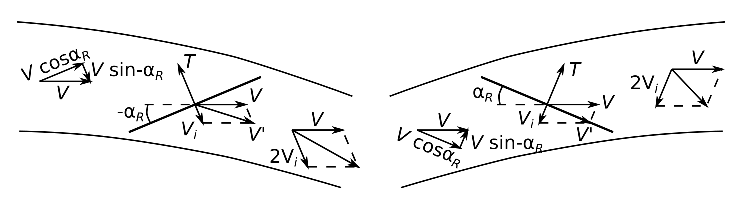
\includegraphics[width=120mm]{images/momentum_theory_forward.eps}
  \caption{Flow trough a rotor in forward flight}
\end{figure}

Transforming this equation for induced velocity gives:
\begin{equation}
  \label{eq-aero-lambda-i-3}
  V_i = \frac{T}{ 2 \rho A_R V' }
\end{equation}

Where $V'$ is the resultant velocity at the rotor.
\begin{equation}
  \label{eq-aero-vel-rotor}
  V' = \sqrt{
    V^2 \cos^2 \alpha_R
    + \left( V \sin \alpha_R - V_i \right)^2
  }
\end{equation}

Writing velocities in normalized form:
\begin{align}
  \label{eq-aero-lambda-i-4}
  \lambda_i &= \frac{V_i}    { \Omega_R R } \\
  \label{eq-aero-mu-x}
  \mu_X     &= \frac{u_{rw}} { \Omega_R R } \\
  \label{eq-aero-mu-z}
  \mu_Z     &= \frac{w_{rw}} { \Omega_R R }
\end{align}

Where:
\begin{align}
  u_{rw} &= V \cos \alpha_R \\
  w_{rw} &= V \sin \alpha_R
\end{align}

Substituting equations (\ref{eq-aero-lambda-i-4}), (\ref{eq-aero-mu-x}), (\ref{eq-aero-mu-z}) and (\ref{eq-aero-vel-rotor}) into (\ref{eq-aero-lambda-i-3}) formula for the normalized induced velocity can be expressed as follows.
\begin{equation}
  \label{eq-aero-lambda-i-5}
  \lambda_i
  =
  \frac{C_T}{ 2 \sqrt{ \mu_X^2 + \left( \mu_Z - \lambda_i \right)^2 } }
\end{equation}

In high speed flight summing helicopter translational velocity and velocity due to rotor shaft rotation causes strong non-uniformities of rotor induced velocity. Glauert’s model is used to describe this phenomena. \cite{Padfield2007, Bramwell2001}
\begin{equation}
  \lambda_i \left( r, \Psi \right)
  =
  \lambda_{i0} + \frac{r}{R} \lambda_{1c} \cos \Psi
\end{equation}

Where:
\begin{align}
  \lambda_{1c} &= \lambda_{i0} \tan \left( \frac{\chi}{2} \right)
  \mathrm{~for~} \chi < \frac{\pi}{2} \\
  \lambda_{1c} &= \lambda_{i0} \cot \left( \frac{\chi}{2} \right)
  \mathrm{~for~} \chi > \frac{\pi}{2}
\end{align}

The wake angle is given by the following formula:
\begin{equation}
  \chi = \arctan \left( \frac{\mu}{ \lambda_{i0} - \mu_Z } \right)
\end{equation}

Where $\lambda_{i0}$ is given by formula (\ref{eq-aero-lambda-i-5}).

\section{Forces Acting on the Blade Segment}

Determining forces and moments acting on segment of the blade is made, assuming that blade is composed of aerodynamically independent, narrow strips of elements. \cite{Stepniewski1984} High aspect ratio of the blade justifies usage of two-dimensional flow, while lift loss at the blade tip and root can be accounted by using tip-loss factor. \cite{Padfield2007, Stepniewski1984, Bramwell2001}

Control-Wind Axis System is used to determine forces and moments generated by the rotor, such computed forces and moments are the transformed to the Body Axis System.

\begin{figure}[h!]
  \centering
  \includegraphics[width=120mm]{images/blade_element_theory_01.eps}
  \caption{Rotor blade element}
\end{figure}

Lift and drag acting on a blade section is given by the following expressions:
\begin{align}
  \label{eq-aero-blade-section-lift}
  dL &= \frac{1}{2} \rho U^2 \left( r, \Psi \right) C_L c_b dr \\
  \label{eq-aero-blade-section-drag}
  dD &= \frac{1}{2} \rho U^2 \left( r, \Psi \right) C_D c_b dr
\end{align}

Lift and drag coefficients are given as follows: \cite{Padfield2007}
\begin{align}
  \label{eq-aero-blade-section-lift-coef}
  C_L &= a \alpha_{BE} \left( r, \Psi \right) \\
  C_D &= \delta_0 + \delta_2 C_T^2
\end{align}

Blade section angle of attack is given by the following formula.
\begin{equation}
  \alpha_{BE} \left( r , \Psi \right) = \theta + \phi \left( r , \Psi \right) 
\end{equation}

Where:
\begin{equation}
  \phi \left( r , \Psi \right)
  =
  \arctan \frac{ U_P \left( r, \Psi \right) }{ U_T \left( r, \Psi \right) }
\end{equation}

Linear velocity of the rotor hub and angular velocity expressed Rotor Axis System are given by the following formulas: \cite{Stepniewski1984, Bramwell2001}
\begin{align}
  {\vec V}_{RH,r}
  &=
  {\boldsymbol T} \left( \varepsilon \right)
  \left(
    {\vec V}_{O,b} + {\vec \omega}_b \times {\vec r}_{RH,b}
  \right) \\
  {\vec \omega}_r
  &=
  {\boldsymbol T} \left( \varepsilon \right)
  {\vec \omega}_b
\end{align}

Rotattion matrix ${\boldsymbol T} \left( \varepsilon \right)$ is given as:
\begin{equation}
  {\boldsymbol T} \left( \varepsilon \right)
  =
  \left[
    \begin{matrix}
       \cos \varepsilon & 0 & \sin \varepsilon \\
                        0 & 1 &              0 \\
      -\sin \varepsilon & 0 & \cos \varepsilon \\
    \end{matrix}
  \right]
\end{equation}

\begin{figure}
  \centering
  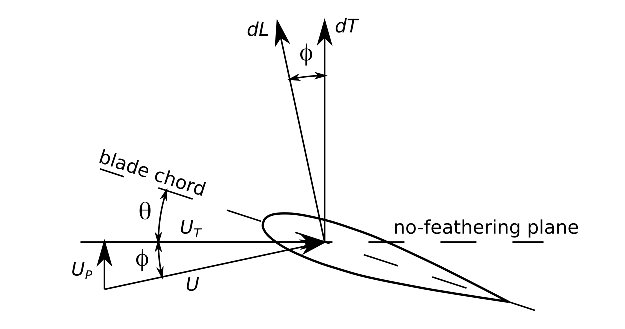
\includegraphics[width=100mm]{images/blade_element_theory_02.eps}
  \caption{Velocity components at the blade element}
\end{figure}

Following formulas can be used to transform this values to Control Axis System:
\begin{align}
  {\vec V}_{RH,c} 
  &=
  {\boldsymbol T} \left( \theta_{1c}, \theta_{1s} \right)
  {\vec V}_{RH,r} \\
  {\vec \omega}_c
  &=
  {\boldsymbol T} \left( \theta_{1c}, \theta_{1s} \right)
  {\vec \omega}_r
\end{align}

Where rotation matrices are:

--- for counterclockwise direction of rotor:
\begin{equation}
  {\boldsymbol T} \left( \theta_{1c}, \theta_{1s} \right)
  =
  \left[
    \begin{matrix}
      1 &                0 &                 0 \\
      0 & \cos \theta_{1c} & -\sin \theta_{1c} \\
      0 & \sin \theta_{1c} &  \cos \theta_{1c} \\
    \end{matrix}
  \right]
  \left[
    \begin{matrix}
      \cos \theta_{1s} & 0 & -\sin \theta_{1s} \\
                    0 & 1 &                 0 \\
      \sin \theta_{1s} & 0 &  \cos \theta_{1s} \\
    \end{matrix}
  \right]
\end{equation}

--- for clockwise direction of rotor:
\begin{equation}
  {\boldsymbol T} \left( \theta_{1c}, \theta_{1s} \right)
  =
  \left[
    \begin{matrix}
      1 &                 0 &                0 \\
      0 &  \cos \theta_{1c} & \sin \theta_{1c} \\
      0 & -\sin \theta_{1c} & \cos \theta_{1c} \\
    \end{matrix}
  \right]
  \left[
    \begin{matrix}
      \cos \theta_{1s} & 0 & -\sin \theta_{1s} \\
                    0 & 1 &                 0 \\
      \sin \theta_{1s} & 0 &  \cos \theta_{1s} \\
    \end{matrix}
  \right]
\end{equation}

Following formulas can be used to transform linear and angular velocity vector to Control-Wind Axis System:
\begin{align}
  {\vec V}_{RH,cw}
  &=
  {\boldsymbol T} \left( \beta \right) {\vec V}_{RH,c} \\
  {\vec \omega}_{cw}
  &=
  {\boldsymbol T} \left( \beta \right) {\vec \omega}_c
\end{align}

Rotation matrix ${\boldsymbol T} \left( \beta \right)$ is given by formula (\ref{eq-aero-matrix-beta}).

Assuming that flapping angle is positive upwards and writing velocity components as:
\begin{align}
  {\vec V}_{RH,cw} &= \left[ u_{cw}, 0, w_{cw} \right]^T \\
  {\vec \omega}_{cw} &= \left[ p_{cw}, q_{cw}, 0 \right]^T
\end{align}

\begin{figure}
  \centering
  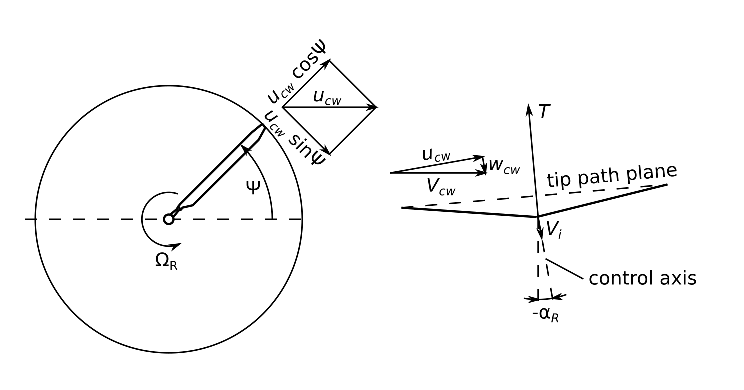
\includegraphics[width=120mm]{images/blade_element_velocity.eps}
  \caption{Air velocities at the blade element}
\end{figure}

Air velocity at the blade segment is:

--- for counterclockwise direction of rotor:
\begin{gather}
  U_T = \Omega_R r \cos \beta + u_{cw} \sin \Psi \\
  \begin{multlined}[0.88\textwidth]
    U_P =
    w_{cw} \cos \beta - V_i \cos \beta
    - \dot \beta r - u_{cw} \sin \beta \cos \Psi \\
    + p_{cw} r \sin \Psi + q_{cw} r \cos \Psi
  \end{multlined}
\end{gather}

--- for clockwise direction of rotor:
\begin{gather}
  U_T = \Omega_R r \cos \beta + u_{cw} \sin \Psi \\
  \begin{multlined}[0.88\textwidth]
    U_P =
    w_{cw} \cos \beta - V_i \cos \beta
    - \dot \beta r - u_{cw} \sin \beta \cos \Psi \\
    - p_{cw} r \sin \Psi + q_{cw} r \cos \Psi
  \end{multlined}
\end{gather}

Assuming that for small angles:
\begin{align}
  \label{eq-aero-sin-beta-approx}
  \sin \beta \approx \beta \\
  \label{eq-aero-cos-beta-approx}
  \cos \beta \approx 1
\end{align}

This expressions can be simplified to:

--- for counterclockwise direction of rotor:
\begin{align}
  U_T &= \Omega_R r + u_{cw} \sin \Psi \\
  U_P &=
  w_{cw} - V_i - \dot \beta r - u_{cw} \beta \cos \Psi
  + p_{cw} r \sin \Psi + q_{cw} r \cos \Psi
\end{align}

--- for clockwise direction of rotor:
  \begin{align}
    U_T &= \Omega_R r + u_{cw} \sin \Psi \\
    U_P &=
    w_{cw} - V_i - \dot \beta r - u_{cw} \beta \cos \Psi
    - p_{cw} r \sin \Psi + q_{cw} r \cos \Psi
  \end{align}

Using normalized velocities:

\begin{align}
  \mu     &= \frac{u_{cw}}{\Omega_R R} \\
  \lambda &= \frac{w_{cw} - V_i}{\Omega_R R}
\end{align}

Expressions for air velocity at the blade segment can be written in the following form:

--- for counterclockwise direction of rotor:
\begin{align}
  U_T &= \Omega_R r + \mu \Omega_R R \sin \Psi \\
  U_P &=
  \lambda \Omega_R R - \dot \beta r - \mu \Omega_R R \beta \cos \Psi
  + p_{cw} r \sin \Psi + q_{cw} r \cos \Psi
\end{align}

--- for clockwise direction of rotor:
\begin{align}
  U_T &= \Omega_R r + \mu \Omega_R R \sin \Psi \\
  U_P &=
  \lambda \Omega_R R - \dot \beta r - \mu \Omega_R R \beta \cos \Psi
  - p_{cw} r \sin \Psi + q_{cw} r \cos \Psi
\end{align}

\section{Rotor Thrust}

Assuming that for small angles:
\begin{align}
  \label{eq-aero-approx-phi}
  \phi = \arctan &\frac{U_P}{U_T} \approx \frac{U_P}{U_T} \\
  \label{eq-aero-approx-u}
  U  &\approx U_T \\
  \label{eq-aero-approx-dt}
  dT &\approx dL
\end{align}

Expression for the blade segment angle of attack is given as follows:
\begin{equation}
  \alpha_{BE} = \theta + \frac{U_P}{U_T}
\end{equation}

Then expression (\ref{eq-aero-blade-section-lift-coef}) can be written as. \cite{GessowMyers1985}
\begin{equation}
  \label{eq-aero-rotor-list-coef}
  C_L = a \left( \theta + \frac{U_P}{U_T} \right)
\end{equation}

Substituting expression (\ref{eq-aero-blade-section-lift}) and taking into account simplifications (\ref{eq-aero-approx-phi}), (\ref{eq-aero-approx-u}) and (\ref{eq-aero-approx-dt}) then rotor thrust is given by the following formula.
\begin{equation}
  dT
  \approx
  \frac{1}{2} \rho a c_b U_T^2 \left( \theta + \frac{U_P}{U_T} \right) dr
\end{equation}

Transforming this relationship gives:
\begin{equation}
  \label{eq-aero-blade-section-thrust}
  dT
  \approx
  \frac{1}{2} \rho a c_b
  \left( \theta U_T^2 + U_P U_T \right) dr
\end{equation}

Total thrust generated by the rotor of $n_b$ blades can be determined by integrating differential equation (\ref{eq-aero-blade-section-thrust}) first with respect to the azimuth then along the blade span. \cite{GessowMyers1985} Total thrust is given as follows:
\begin{equation}
  \label{eq-aero-thrust-2}
  T = \frac{ n_b }{ 2 \pi } \int_{0}^{2 \pi} \int_{0}^{BR}
  \frac{dT}{dr} dr d\Psi
\end{equation}

Where $B$ is a tip loss factor.

Substituting (\ref{eq-aero-blade-section-thrust}) into (\ref{eq-aero-thrust-2}) gives:
\begin{equation}
  T = \frac{1}{2} \rho a c_b n_b
  \left(
  \theta \frac{1}{2 \pi}
  \int_{0}^{2\pi} \int_{0}^{BR} \frac{U_T^2}{dr} dr d\Psi
  +
  \frac{1}{2\pi} \int_{0}^{2\pi} \int_{0}^{BR} U_P U_T dr d\Psi
  \right)
\end{equation}

Neglecting helicopter angular velocity expressions for $U_T^2$ and $U_P U_T$ can be written as:
\begin{gather}
  \label{eq-aero-u-t-sq}
  U_T^2 =
  r^2 \Omega_R^2 + 2 \Omega_R^2 R r \mu \sin \Psi
  + \mu^2 R^2 \Omega_R^2 \sin^2 \Psi \\
  \label{eq-aero-u-p-u-t}
  \begin{multlined}[0.88\textwidth]
  U_P U_T =
  \lambda \Omega_R^2 R r - \dot \beta \Omega_R r^2
  - \beta \mu \Omega_R^2 R r \cos \Psi \\
  + \lambda \mu \Omega_R^2 R^2 \sin \Psi
  - \dot \beta \mu \Omega_R R r \sin \Psi
  - \beta \mu^2 \Omega_R^2 R^2 \sin \Psi \cos \Psi
  \end{multlined}
\end{gather}

Expression for the blade flapping angle can be written as follows: \cite{Padfield2007, GessowMyers1985, NASA-TT-F-494}
\begin{equation}
  \label{eq-aero-blade-flapping-angle}
  \beta \left( \Psi \right) = 
  \beta_0 + \beta_{1c} \cos \Psi + \beta_{1s} \sin \Psi
\end{equation}

Assuming constant rotor revolution speed, blade flapping angle derivatives with respect to time can be written as derivatives with respect to the azimuth. \cite{GessowMyers1985}
\begin{gather}
  \dot \beta = \frac{d\beta}{dt}
  = \frac{d\beta}{d\Psi} \frac{d\Psi}{dt} =
  \bar \beta \Omega_R =
  \Omega_R
  \left( \beta_{1s} \cos \Psi - \beta_{1c} \sin \Psi \right) \\
  \ddot \beta = \frac{d^2\beta}{dt^2}
  = \frac{d^2\beta}{d\Psi^2} \left( \frac{d\Psi}{dt} \right)^2 = 
  \bar{\bar \beta} \Omega_R^2
  =
  -\Omega_R^2
  \left( \beta_{1c} \cos \Psi + \beta_{1s} \sin \Psi \right)
\end{gather}

Then expressions for $U_T^2$ and $U_P U_T$ can be written as:
\begin{gather}
  U_T^2 = r^2 \Omega_R^2 + 2 \Omega_R^2 R r \mu \sin \Psi
  + \mu^2 R^2 \Omega_R^2 \sin^2 \Psi \\
  \begin{multlined}[0.88\textwidth]
    U_P U_T = \lambda \Omega_R^2 R r
    - \beta_{1s} \Omega_R^2 r^2 \cos \Psi
    + \beta_{1c} \Omega_R^2 r^2 \sin \Psi \\
    - \beta \mu \Omega_R^2 R r \cos \Psi
    + \lambda \mu \Omega_R^2 R^2 \sin \Psi
    - \beta_{1s} \mu \Omega_R^2 R r \sin \Psi \cos \Psi \\
    + \beta_{1c} \mu \Omega_R^2 R r \sin^2 \Psi
    - \beta \mu^2 \Omega_R^2 R^2 \sin \Psi \cos \Psi
  \end{multlined}
\end{gather}

Knowing that: \cite{GessowMyers1985}
\begin{gather}
  \frac{1}{2\pi} \int_{0}^{2\pi} \sin \Psi d\Psi =
  \frac{1}{2\pi} \int_{0}^{2\pi} \cos \Psi d\Psi = 0 \\
  \frac{1}{2\pi} \int_{0}^{2\pi} \sin^2 \Psi d\Psi =
  \frac{1}{2\pi} \int_{0}^{2\pi} \cos^2 \Psi d\Psi = \frac{1}{2} \\
  \frac{1}{2\pi} \int_{0}^{2\pi} \sin \Psi \cos \Psi d\Psi = 0
\end{gather}

Rotor thrust can be written as:
\begin{equation}
  T = \frac{1}{2} \rho a c_b n_b \Omega_R^2 R^3 B
  \left[
    \frac{\lambda B}{2} 
    +
    \frac{\theta}{3} \left( B^2 + \frac{3}{2} \mu^2 \right)
    +
    \frac{\beta_{1c} B}{4} \mu
  \right]
\end{equation}

Using expression (\ref{eq-aero-thrust-coef}) rotor thrust coefficient is given by the following formula:
\begin{equation}
  C_T = \frac{1}{2} a s B
  \left[
    \frac{\lambda B}{2}
    +
    \frac{\theta}{3} \left( B^2 + \frac{3}{2} \mu^2 \right)
    +
    \frac{\beta_{1c} B}{4} \mu
  \right]
\end{equation}

Where $s$ is rotor solidity.

\section{Rotor Torque}

The torque on a blade element is given by the following formula. \cite{GessowMyers1985, Bramwell2001}
\begin{equation}
  \label{eq-aero-blade-section-torque}
  dQ = r \left( dD \cos \phi - dL \sin \phi \right) dr
\end{equation}

Assuming that for small angles:
\begin{align}
  \sin \phi &\approx \phi \\
  \cos \phi &\approx 1
\end{align}

And assuming that drag coefficient is constant along blade span, expression (\ref{eq-aero-blade-section-torque}) can be written as: \cite{GessowMyers1985, Bramwell2001}
\begin{equation}
  dQ =
  \frac{1}{2} \rho U_T^2 C_D c_b r dr -
  \frac{1}{2} \rho U_T^2 C_L c_b r \phi dr
\end{equation}

Torque due to the profile drag can be expressed as: \cite{Bramwell2001}
\begin{equation}
  Q_p = \frac{n_b}{2\pi}
  \int_{0}^{R} \int_{0}^{2\pi} \frac{1}{2} \rho U_T^2 C_D c_b r d \Psi dr
\end{equation}

Substituting (\ref{eq-aero-u-t-sq}) and integrating this equation first with respect to the azimuth then along the blade span gives:
\begin{equation}
  Q_p = \frac{1}{2} \rho n_b c_b \Omega_R^2 R^4 C_D
  \left( \frac{1}{4} + \frac{1}{4} \mu^2 \right)
\end{equation}

Induced torque is given by the following formula: \cite{Bramwell2001}
\begin{equation}
  Q_i = \frac{n_b}{2\pi} \int_{0}^{R} \int_{0}^{2\pi}
  \frac{1}{2} \rho U_T^2 C_L c_b r \phi d \Psi dr
\end{equation}

Substituting (\ref{eq-aero-approx-phi}) and (\ref{eq-aero-rotor-list-coef}) gives:
\begin{equation}
  \label{eq-aero-q-i}
  Q_i = \frac{n_b}{2\pi} \frac{1}{2} \rho a c_b
  \int_{0}^{R} \int_{0}^{2\pi}
  \left( \theta U_P U_T r + U_P^2 r \right) d \Psi dr
\end{equation}

Neglecting helicopter angular velocity expressions for $U_P^2$ can be written as:
\begin{multline}
  \label{eq-aero-u-p-sq}
  U_P^2 = \dot \beta^2 r^2
  + 2 \beta \dot \beta \mu \Omega_R R r \cos \Psi
  - 2 \dot \beta \lambda \Omega_R R r \\
  + \beta^2 \mu^2 \Omega_R^2 R^2 \cos^2 \Psi
  - 2 \beta \lambda \mu \Omega_R^2 R^2 \cos \Psi
  + \lambda^2 \Omega_R^2 R^2
\end{multline}

Substituting (\ref{eq-aero-u-p-u-t}) and (\ref{eq-aero-u-p-sq}) into (\ref{eq-aero-q-i}) and integrating equation (\ref{eq-aero-q-i}) first with respect to the azimuth then along the blade span gives:
\begin{multline}
Q_i = \frac{1}{2} \rho a c_b n_b \Omega_R^2 R^4
\left[
    \frac{1}{3} \lambda \theta
  + \frac{1}{2} \lambda^2
  - \frac{1}{8} \left( \beta_{1c}^2 + \beta_{1s}^2 \right)
  \right.
  \\
  \left.
  + \frac{1}{2} \mu^2
  \left(
    \frac{\beta_0^2}{2}
    - \frac{3}{8} \beta_{1c}^2
    - \frac{1}{8} \beta_{1s}^2
  \right)
  - \frac{1}{2} \mu \lambda \beta_{1c}
  + \frac{1}{3} \mu \beta_0 \beta_{1s}
\right]
\end{multline}

The total rotor torque is given as follows: \cite{Bramwell2001, NASA-TT-F-494}
\begin{gather}
  Q = Q_p - Q_i \\
  \begin{multlined}[0.88\textwidth]
    Q = \frac{1}{2} \rho a c_b n_b \Omega_R^2 R^4
    \left[
      \frac{C_D}{4a} \left( 1 + \mu^2 \right)
      - \frac{1}{3} \lambda \theta
      - \frac{1}{2} \lambda^2
      + \frac{1}{8} \left( \beta_{1c}^2 + \beta_{1s}^2 \right)
      \right.
      \\
      \left.
      - \frac{1}{2} \mu^2
      \left(
        \frac{\beta_0^2}{2}
        - \frac{3}{8} \beta_{1c}^2
        - \frac{1}{8} \beta_{1s}^2
      \right)
      + \frac{1}{2} \mu \lambda \beta_{1c}
      - \frac{1}{3} \mu \beta_0 \beta_{1s}
    \right]
  \end{multlined}
\end{gather}

Rotor torque coefficient can be written as:
\begin{multline}
  C_Q = \frac{1}{2} a s
  \left[
    \frac{C_D}{4a} \left( 1 + \mu^2 \right)
    - \frac{1}{3} \lambda \theta
    - \frac{1}{2} \lambda^2
    + \frac{1}{8} \left( \beta_{1c}^2 + \beta_{1s}^2 \right)
    \right.
    \\
    \left.
    - \frac{1}{2} \mu^2
    \left(
      \frac{\beta_0^2}{2}
      - \frac{3}{8} \beta_{1c}^2
      - \frac{1}{8} \beta_{1s}^2
    \right)
    + \frac{1}{2} \mu \lambda \beta_{1c}
    - \frac{1}{3} \mu \beta_0 \beta_{1s}
  \right]
\end{multline}

\section{Flapping Coefficients}

Expressions for blades flapping coefficients can be derived from the equation of moments equilibrium about flapping hinge using method described in \cite{NASA-TT-F-494}.

\begin{figure}
  \centering
  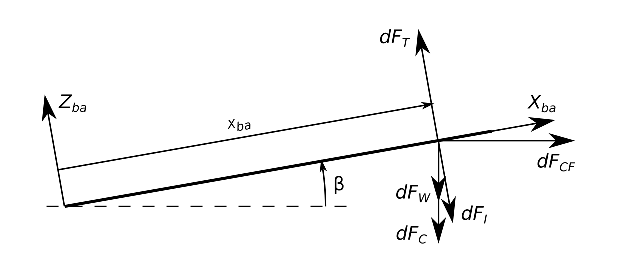
\includegraphics[width=100mm]{images/blade_element_moments.eps}
  \caption{Forces acting on the blade element}
\end{figure}

\begin{minipage}{\textwidth}
  Moments equilibrium about flapping hinge can be written as follows: \cite{GessowMyers1985}
  \begin{equation}
    \label{eq-aero-blade-moments-equilibrium}
    M_I + M_{CF} + M_C + M_T + M_W = 0
  \end{equation}

  Where:
  \begin{description}[align=right,labelwidth=1.5cm]
    \item [$M_I$]    [N$\cdot$m] moment due to inertia forces of flapping
    \item [$M_{CF}$] [N$\cdot$m] moment due to centrifugal force
    \item [$M_C$]    [N$\cdot$m] moment due to Coriolis force
    \item [$M_T$]    [N$\cdot$m] moment due to thrust
    \item [$M_W$]    [N$\cdot$m] moment due to weight
  \end{description}
\end{minipage}

\subsection{Moments of Inertia Forces}

Assuming that rotor revolution speed is constant, helicopter angular velocities are constant and rotor blades are able to move about flapping hinge axis while neglecting helicopter yaw motion and blades pitching and lagging motion then centrifugal force can be written as:
\begin{equation}
  dF_{CF} = m_b \Omega_R^2 r dr
\end{equation}

Component of the Coriolis force laying on the flapping plane is given:

--- for counterclockwise direction of rotor:
\begin{equation}
  dF_C =
    2 m_b p_{cw} \Omega_R r \cos \Psi dr
  - 2 m_b q_{cw} \Omega_R r \sin \Psi dr
\end{equation}

--- for clockwise direction of rotor:
\begin{equation}
  dF_C =
  - 2 m_b p_{cw} \Omega_R r \cos \Psi dr
  - 2 m_b q_{cw} \Omega_R r \sin \Psi dr
\end{equation}

Moment of inertia forces of flapping is given by the following formula:
\begin{equation}
  M_I = - \ddot \beta \int_{0}^{R} m_b r^2 dr
\end{equation}

Assuming that rotor blades are homogeneous rods blade first moment of mass and moment of inertia can be written as: \cite{NASA-TT-F-494}
\begin{align}
  \label{eq-aero-j-b}
  J_b &\approx \int_{0}^{R} m_b r^2 dr \\
  \label{eq-aero-s-b}
  S_b &\approx \int_{0}^{R} m_b r dr
\end{align}

Hence:
\begin{equation}
  M_I = - \ddot \beta J_b
\end{equation}

Taking into account (\ref{eq-aero-sin-beta-approx}) and (\ref{eq-aero-cos-beta-approx}) moment of centrifugal forces is:
\begin{equation}
  \label{eq-aero-m-cf}
  M_{CF} =
  - \int_{0}^{R} \beta m_b \Omega_R^2 r^2 dr =
  - \Omega_R^2 \beta \int_{0}^{R} m_b r^2 dr
\end{equation}

Substituting (\ref{eq-aero-j-b}) into (\ref{eq-aero-m-cf}) gives:
\begin{equation}
  M_{CF} = - \Omega_R^2 \beta J_b
\end{equation}

Moment of Coriolis forces can be writes as:

--- for counterclockwise direction of rotor:
\begin{multline}
  M_C =
    2 \int_{0}^{R} m_b p_{cw} \Omega_R r^2 \cos \Psi dr
  - 2 \int_{0}^{R} m_b q_{cw} \Omega_R r^2 \sin \Psi dr
  = \\ =
  2 p_{cw} \Omega_R J_b \cos \Psi - 2 q_{cw} \Omega_R J_b \sin \Psi
\end{multline}

--- for clockwise direction of rotor:
\begin{multline}
  M_C =
  - 2 \int_{0}^{R} m_b p_{cw} \Omega_R r^2 \cos \Psi dr
  - 2 \int_{0}^{R} m_b q_{cw} \Omega_R r^2 \sin \Psi dr
  = \\ =
  -2 p_{cw} \Omega_R J_b \cos \Psi - 2 q_{cw} \Omega_R J_b \sin \Psi
\end{multline}

Using approximation (\ref{eq-aero-s-b}) moment due to weight can expressed as:
\begin{equation}
  M_W = -g \int_{0}^{R} m_b r dr = -g S_b
\end{equation}

\subsection{Moment of Thrust}

Using equation (\ref{eq-aero-blade-section-thrust}) expression for moment of thrust about flapping hinge can be written as follows:
\begin{equation}
  M_T =
  \int_{0}^{BR} dT r = 
  \frac{1}{2} \rho a c_b
  \int_{0}^{BR} \left( \theta U_T^2 + U_P U_T \right) dr
\end{equation}

\subsection{Equilibrium of Moments about Flapping Hinge}

Substituting into (\ref{eq-aero-blade-moments-equilibrium}) expressions for moments of thrust, weight, inertia, centrifugal and Coriolis forces moments equilibrium equation is given as:

--- for counterclockwise direction of rotor:
\begin{gather}
  \begin{multlined}[0.88\textwidth]
    \int_{0}^{BR} dT r
    - \ddot \beta J_b
    - \beta \Omega_R^2 J_b
    + 2 p_{cw} \Omega_R J_b \cos \Psi \\
    - 2 q_{cw} \Omega_R J_b \sin \Psi
    - g S_b
    = 0
  \end{multlined}
  \\
  \begin{multlined}[0.88\textwidth]
    \label{eq-aero-equilibrium-blade-moments-ccw-1}
    - J_b \ddot \beta
    - J_b \beta \Omega_R^2
    + \int_{0}^{BR} dT r
    = 2 J_b q_{cw} \Omega_R \sin \Psi \\
    - 2 J_b p_{cw} \Omega_R \cos \Psi
    + g S_b
  \end{multlined}
\end{gather}
  
--- for clockwise direction of rotor:
\begin{gather}
  \begin{multlined}[0.88\textwidth]
    \int_{0}^{BR} dT r
    - \ddot \beta J_b
    - \beta \Omega_R^2 J_b
    - 2 p_{cw} \Omega_R J_b \cos \Psi \\
    - 2 q_{cw} \Omega_R J_b \sin \Psi
    - g S_b
    = 0
  \end{multlined}
  \\
  \begin{multlined}[0.88\textwidth]
    \label{eq-aero-equilibrium-blade-moments-cw-1}
    - J_b \ddot \beta
    - J_b \beta \Omega_R^2
    + \int_{0}^{BR} dT r
    = 2 J_b q_{cw} \Omega_R \sin \Psi \\
    + 2 J_b p_{cw} \Omega_R \cos \Psi
    + g S_b
  \end{multlined}
\end{gather}

Dividing both sides of equations (\ref{eq-aero-equilibrium-blade-moments-ccw-1}) and (\ref{eq-aero-equilibrium-blade-moments-cw-1}) by $J_b \Omega_R^2$ gives:
\begin{gather}
  \label{eq-aero-equilibrium-blade-moments-ccw-2}
  \bar{\bar \beta} + \beta
  = \frac{1}{ J_b \Omega_R^2 } \int_{0}^{BR} dT r
  - 2 \frac{q_{cw}}{\Omega_R} \sin \Psi
  + 2 \frac{p_{cw}}{\Omega_R} \cos \Psi
  - \frac{g S_b}{J_b \Omega_R^2} \\
  \label{eq-aero-equilibrium-blade-moments-cw-2}
    \bar{\bar \beta} + \beta
  = \frac{1}{ J_b \Omega_R^2 } \int_{0}^{BR} dT r
  - 2 \frac{q_{cw}}{\Omega_R} \sin \Psi
  - 2 \frac{p_{cw}}{\Omega_R} \cos \Psi
  - \frac{g S_b}{J_b \Omega_R^2}
\end{gather}

Substituting expressions (\ref{eq-aero-u-t-sq}) and (\ref{eq-aero-u-p-u-t}) into (\ref{eq-aero-equilibrium-blade-moments-ccw-2}) and (\ref{eq-aero-equilibrium-blade-moments-cw-2}) gives:
\begin{multline}
  \label{eq-aero-blade-moment-thrust-ccw}
  M_T =
  \int_{0}^{BR} dT r =
  \frac{1}{2} \rho a c_b
  \int_{0}^{BR} \left( \theta U_T^2 + U_P U_T \right) r dr = \\
  =
  \frac{1}{2} \rho a c_b R^4 \Omega_R^2
  \left(
    \frac{B^4}{4} \theta
  + \frac{2}{3} B^3 \theta \mu \sin \Psi
  + \frac{B^2}{2} \theta \mu^2 \sin^2 \Psi
  \right.
  \\
  + \frac{B^3}{3} \lambda
  - \frac{B^4}{4} \bar \beta
  - \frac{B^3}{3} \beta \mu \cos \Psi
  + \frac{B^4}{4} \frac{p_{cw}}{\Omega_R} \sin \Psi \\
  + \frac{B^2}{2} \lambda \mu \sin \Psi
  - \frac{B^2}{2} \beta \mu^2 \sin \Psi \cos \Psi
  - \frac{B^3}{3} \bar \beta \mu \sin \Psi
  \\
  \left.
  + \frac{B^3}{3} \frac{p_{cw}}{\Omega_R} \mu \sin^2 \Psi
  + \frac{B^4}{4} \frac{q_{cw}}{\Omega_R} \cos \Psi
  + \frac{B^3}{3} \frac{q_{cw}}{\Omega_R} \mu \sin \Psi \cos \Psi
  \right)
\end{multline}
\begin{multline}
  \label{eq-aero-blade-moment-thrust-cw}
  M_T =
  \int_{0}^{BR} dT r =
  \frac{1}{2} \rho a c_b
  \int_{0}^{BR} \left( \theta U_T^2 + U_P U_T \right) r dr = \\
  =
  \frac{1}{2} \rho a c_b R^4 \Omega_R^2
  \left(
    \frac{B^4}{4} \theta
  + \frac{2}{3} B^3 \theta \mu \sin \Psi
  + \frac{B^2}{2} \theta \mu^2 \sin^2 \Psi
  \right.
  \\
  + \frac{B^3}{3} \lambda
  - \frac{B^4}{4} \bar \beta
  - \frac{B^3}{3} \beta \mu \cos \Psi
  - \frac{B^4}{4} \frac{p_{cw}}{\Omega_R} \sin \Psi \\
  + \frac{B^2}{2} \lambda \mu \sin \Psi
  - \frac{B^2}{2} \beta \mu^2 \sin \Psi \cos \Psi
  - \frac{B^3}{3} \bar \beta \mu \sin \Psi
  \\
  \left.
  - \frac{B^3}{3} \frac{p_{cw}}{\Omega_R} \mu \sin^2 \Psi
  + \frac{B^4}{4} \frac{q_{cw}}{\Omega_R} \cos \Psi
  + \frac{B^3}{3} \frac{q_{cw}}{\Omega_R} \mu \sin \Psi \cos \Psi
  \right)
\end{multline}

Knowing that:
\begin{align}
  \label{eq-aero-trigonometric-4}
  \sin \Psi \cos \Psi &= \frac{ \sin \left( 2 \Psi \right) }{2} \\
  \label{eq-aero-trigonometric-5}
  \sin^2 \Psi &= \frac{ 1 - \cos \left( 2 \Psi \right) }{2} \\
  \label{eq-aero-trigonometric-6}
  \cos^2 \Psi &= \frac{ 1 + \cos \left( 2 \Psi \right) }{2} \\
  \label{eq-aero-trigonometric-7}
  \cos \Psi \sin \left( 2 \Psi \right) &=
  \frac{ \sin \Psi + \sin \left( 3 \Psi \right) }{2} \\
  \label{eq-aero-trigonometric-8}
  \sin \Psi \sin \left( 2 \Psi \right) &=
  \frac{ \cos \Psi - \cos \left( 3 \Psi \right) }{2}
\end{align}

Substituting (\ref{eq-aero-blade-moment-thrust-ccw}) into (\ref{eq-aero-equilibrium-blade-moments-ccw-2}) and (\ref{eq-aero-blade-moment-thrust-cw}) into (\ref{eq-aero-equilibrium-blade-moments-cw-2}) gives:
\begin{multline}
  \label{eq-aero-flapping-coefs-ccw-1}
  \bar{\bar \beta} + \bar \beta \frac{\gamma}{2}
  \left( \frac{B^4}{4} + \frac{B^3}{3} \mu \sin \Psi \right)
  + \beta \left(
    1 + \frac{B^3}{6} \gamma \mu \cos \Psi
    + \frac{B^2}{8} \gamma \mu^2 \sin \left( 2 \Psi \right)
  \right)
  = \\ =
  \frac{\gamma}{2}
  \left(
      \frac{B^3}{3} \lambda
    + \frac{B^4}{4} \frac{p_{cw}}{\Omega_R} \sin \Psi
    + \frac{B^2}{2} \lambda \mu \sin \Psi
    + \frac{B^3}{6} \frac{p_{cw}}{\Omega_R} \mu
    - \frac{B^3}{6} \frac{p_{cw}}{\Omega_R} \mu \cos \left( 2 \Psi \right)
    \right.
    \\
    + \frac{B^4}{4} \frac{q_{cw}}{\Omega_R} \cos \Psi
    + \frac{B^3}{6} \frac{q_{cw}}{\Omega_R} \mu \sin \left( 2 \Psi \right)
    + \frac{B^4}{4} \theta
    \\
    \left.
    + \frac{2}{3} B^3 \theta \mu \sin \Psi
    + \frac{B^2}{4} \theta \mu^2
    - \frac{B^2}{4} \theta \mu^2 \cos \left( 2 \Psi \right)
  \right)
  \\
  - 2 \frac{q_{cw}}{\Omega_R} \sin \Psi
  + 2 \frac{p_{cw}}{\Omega_R} \cos \Psi
  - \frac{ g S_b }{ J_b \Omega_R^2 }
\end{multline}
\begin{multline}
  \label{eq-aero-flapping-coefs-cw-1}
  \bar{\bar \beta} + \bar \beta \frac{\gamma}{2}
  \left( \frac{B^4}{4} + \frac{B^3}{3} \mu \sin \Psi \right)
  + \beta \left(
    1 + \frac{B^3}{6} \gamma \mu \cos \Psi
    + \frac{B^2}{8} \gamma \mu^2 \sin \left( 2 \Psi \right)
  \right)
  = \\ =
  \frac{\gamma}{2}
  \left(
      \frac{B^3}{3} \lambda
    - \frac{B^4}{4} \frac{p_{cw}}{\Omega_R} \sin \Psi
    + \frac{B^2}{2} \lambda \mu \sin \Psi
    - \frac{B^3}{6} \frac{p_{cw}}{\Omega_R} \mu
    + \frac{B^3}{6} \frac{p_{cw}}{\Omega_R} \mu \cos \left( 2 \Psi \right)
    \right.
    \\
    + \frac{B^4}{4} \frac{q_{cw}}{\Omega_R} \cos \Psi
    + \frac{B^3}{6} \frac{q_{cw}}{\Omega_R} \mu \sin \left( 2 \Psi \right)
    + \frac{B^4}{4} \theta
    \\
    \left.
    + \frac{2}{3} B^3 \theta \mu \sin \Psi
    + \frac{B^2}{4} \theta \mu^2
    - \frac{B^2}{4} \theta \mu^2 \cos \left( 2 \Psi \right)
  \right)
  \\
  - 2 \frac{q_{cw}}{\Omega_R} \sin \Psi
  - 2 \frac{p_{cw}}{\Omega_R} \cos \Psi
  - \frac{ g S_b }{ J_b \Omega_R^2 }
\end{multline}

Where $\gamma$ is a blade Lock number.

Transforming equations (\ref{eq-aero-flapping-coefs-ccw-1}) and (\ref{eq-aero-flapping-coefs-cw-1}) gives:
\begin{multline}
  \label{eq-aero-flapping-coefs-ccw-2}
  \bar{\bar \beta} + \bar \beta \frac{\gamma}{2}
  \left( \frac{B^4}{4} + \frac{B^3}{3} \mu \sin \Psi \right)
  + \beta \left(
    1 + \frac{B^3}{6} \gamma \mu \cos \Psi
    + \frac{B^2}{8} \gamma \mu^2 \sin \left( 2 \Psi \right)
  \right)
  = \\ =
  \left[
    \frac{\gamma}{2}
    \left(
        \frac{B^3}{3} \lambda
      + \frac{B^3}{6} \frac{p_{cw}}{\Omega_R} \mu
      + \frac{B^4}{4} \theta
      + \frac{B^2}{4} \theta \mu^2
    \right)
    - \frac{ g S_b }{ J_b \Omega_R^2 }
  \right]
  \\
  + \left[
    \frac{\gamma}{2}
    \left( \frac{B^4}{4} \frac{q_{cw}}{\Omega_R} \right)
    + 2 \frac{p_{cw}}{\Omega_R}
  \right] \cos \Psi
  \\
  + \left[
    \frac{\gamma}{2}
    \left(
        \frac{B^4}{4} \frac{p_{cw}}{\Omega_R}
      + \frac{B^2}{2} \lambda \mu
      + \frac{2}{3} B^3 \theta \mu
    \right)
    - 2 \frac{q_{cw}}{\Omega_R}
  \right] \sin \Psi
  \\
  + \left[
    \frac{\gamma}{2}
    \left(
      - \frac{B^3}{6} \frac{p_{cw}}{\Omega_R} \mu
      - \frac{B^2}{4} \theta \mu^2
    \right)
  \right] \cos \left( 2 \Psi \right)
  \\
  + \left[
    \frac{\gamma}{2}
    \left( \frac{B^3}{6} \frac{q_{cw}}{\Omega_R} \mu \right)
  \right] \sin \left( 2 \Psi \right)
\end{multline}

\vfill

\begin{multline}
  \label{eq-aero-flapping-coefs-cw-2}
  \bar{\bar \beta} + \bar \beta \frac{\gamma}{2}
  \left( \frac{B^4}{4} + \frac{B^3}{3} \mu \sin \Psi \right)
  + \beta \left(
    1 + \frac{B^3}{6} \gamma \mu \cos \Psi
    + \frac{B^2}{8} \gamma \mu^2 \sin \left( 2 \Psi \right)
  \right)
  = \\ =
  \left[
    \frac{\gamma}{2}
    \left(
        \frac{B^3}{3} \lambda
      - \frac{B^3}{6} \frac{p_{cw}}{\Omega_R} \mu
      + \frac{B^4}{4} \theta
      + \frac{B^2}{4} \theta \mu^2
    \right)
    - \frac{ g S_b }{ J_b \Omega_R^2 }
  \right]
  \\
  + \left[
    \frac{\gamma}{2}
    \left( \frac{B^4}{4} \frac{q_{cw}}{\Omega_R} \right)
    - 2 \frac{p_{cw}}{\Omega_R}
  \right] \cos \Psi
  \\
  + \left[
    \frac{\gamma}{2}
    \left(
      - \frac{B^4}{4} \frac{p_{cw}}{\Omega_R}
      + \frac{B^2}{2} \lambda \mu
      + \frac{2}{3} B^3 \theta \mu
    \right)
    - 2 \frac{q_{cw}}{\Omega_R}
  \right] \sin \Psi
  \\
  + \left[
    \frac{\gamma}{2}
    \left(
        \frac{B^3}{6} \frac{p_{cw}}{\Omega_R} \mu
      - \frac{B^2}{4} \theta \mu^2
    \right)
  \right] \cos \left( 2 \Psi \right)
  \\
  + \left[
    \frac{\gamma}{2}
    \left( \frac{B^3}{6} \frac{q_{cw}}{\Omega_R} \mu \right)
  \right] \sin \left( 2 \Psi \right)
\end{multline}

\vfill

Differentiating equation (\ref{eq-aero-blade-flapping-angle}) gives:
\begin{align}
  \label{eq-aero-beta-prim}
  \bar \beta &=
  \left( \beta_{1s} \cos \Psi - \beta_{1c} \sin \Psi \right) \\
  \label{eq-aero-beta-bis}
  \bar{\bar \beta} &= -
  \left( \beta_{1c} \cos \Psi + \beta_{1s} \sin \Psi  \right)
\end{align}

Substituting expressions (\ref{eq-aero-beta-prim}) and (\ref{eq-aero-beta-bis}) into equations (\ref{eq-aero-flapping-coefs-ccw-2}) and (\ref{eq-aero-flapping-coefs-cw-2}) as well as using trigonometric identities (\ref{eq-aero-trigonometric-4}), (\ref{eq-aero-trigonometric-5}), (\ref{eq-aero-trigonometric-6}), (\ref{eq-aero-trigonometric-7}) and (\ref{eq-aero-trigonometric-8}) gives:
\begin{gather}
  \label{eq-aero-flapping-coefs-ccw-3}
  \begin{multlined}[0.88\textwidth]
    \beta_0
    + 
    \beta_{1s} \gamma \frac{B^2}{8}
    \left( \frac{\mu^2}{2} + B^2 \right) \cos \Psi
    +
    \beta_{1c} \gamma \frac{B^2}{8}
    \left( \frac{\mu^2}{2} - B^2 \right) \sin \Psi
    \\
    +
    \beta_{1c} \gamma \frac{B^3}{6} \mu \cos \left( 2 \Psi \right)
    +
    \left(
        \beta_{1s} \gamma \frac{B^3}{6} \mu
      + \beta_0 \gamma \frac{B^2}{8} \mu^2
    \right) \sin \left( 2 \Psi \right)
    \\
    +
    \beta_{1c} \gamma \frac{B^2}{16} \mu^2 \sin \left( 3 \Psi \right)
    -
    \beta_{1s} \gamma \frac{B^2}{16} \mu^2 \cos \left( 3 \Psi \right)
    = \\ =
    \left[
      \frac{\gamma}{2}
      \left(
          \frac{B^3}{3} \lambda
        + \frac{B^3}{6} \frac{p_{cw}}{\Omega_R} \mu
        + \frac{B^4}{4} \theta
        + \frac{B^2}{4} \theta \mu^2
      \right) - \frac{ g S_b }{ J_b \Omega_R^2 }
    \right]
    \\
    + \left[
      \frac{\gamma}{2}
      \left(
          \frac{B^4}{4} \frac{q_{cw}}{\Omega_R}
        - \frac{B^3}{3} \beta_0 \mu
      \right) + 2 \frac{p_{cw}}{\Omega_R}
    \right] \cos \Psi
    \\
    + \left[
      \frac{\gamma}{2}
      \left(
          \frac{B^4}{4} \frac{p_{cw}}{\Omega_R}
        + \frac{B^2}{2} \lambda \mu
        + \frac{2}{3} B^3 \theta \mu
        \right) - 2 \frac{q_{cw}}{\Omega_R}
    \right] \sin \Psi
    \\
    + \left[
      \frac{\gamma}{2}
      \left(
        - \frac{B^3}{6} \frac{p_{cw}}{\Omega_R} \mu
        - \frac{B^2}{4} \theta \mu^2
      \right)
    \right] \cos \left( 2 \Psi \right)
    \\
    + \left[
      \frac{\gamma}{2}
      \left( \frac{B^3}{6} \frac{q_{cw}}{\Omega_R} \mu \right)
    \right] \sin \left( 2 \Psi \right)
  \end{multlined}
  \\
  \label{eq-aero-flapping-coefs-cw-3}
  \begin{multlined}[0.88\textwidth]
    \beta_0
    + 
    \beta_{1s} \gamma \frac{B^2}{8}
    \left( \frac{\mu^2}{2} + B^2 \right) \cos \Psi
    +
    \beta_{1c} \gamma \frac{B^2}{8}
    \left( \frac{\mu^2}{2} - B^2 \right) \sin \Psi
    \\
    +
    \beta_{1c} \gamma \frac{B^3}{6} \mu \cos \left( 2 \Psi \right)
    +
    \left(
        \beta_{1s} \gamma \frac{B^3}{6} \mu
      + \beta_0 \gamma \frac{B^2}{8} \mu^2
    \right) \sin \left( 2 \Psi \right)
    \\
    -
    \beta_{1s} \gamma \frac{B^2}{16} \mu^2 \cos \left( 3 \Psi \right)
    +
    \beta_{1c} \gamma \frac{B^2}{16} \mu^2 \sin \left( 3 \Psi \right)
    = \\ =
    \left[
      \frac{\gamma}{2}
      \left(
          \frac{B^3}{3} \lambda
        - \frac{B^3}{6} \frac{p_{cw}}{\Omega_R} \mu
        + \frac{B^4}{4} \theta
        + \frac{B^2}{4} \theta \mu^2
      \right) - \frac{ g S_b }{ J_b \Omega_R^2 }
    \right]
    \\
    + \left[
      \frac{\gamma}{2}
      \left(
          \frac{B^4}{4} \frac{q_{cw}}{\Omega_R}
        - \frac{B^3}{3} \beta_0 \mu
      \right) - 2 \frac{p_{cw}}{\Omega_R}
    \right] \cos \Psi
    \\
    + \left[
      \frac{\gamma}{2}
      \left(
        - \frac{B^4}{4} \frac{p_{cw}}{\Omega_R}
        + \frac{B^2}{2} \lambda \mu
        + \frac{2}{3} B^3 \theta \mu
        \right) - 2 \frac{q_{cw}}{\Omega_R}
    \right] \sin \Psi
    \\
    + \left[
      \frac{\gamma}{2}
      \left(
          \frac{B^3}{6} \frac{p_{cw}}{\Omega_R} \mu
        - \frac{B^2}{4} \theta \mu^2
      \right)
    \right] \cos \left( 2 \Psi \right)
    \\
    + \left[
      \frac{\gamma}{2}
      \left( \frac{B^3}{6} \frac{q_{cw}}{\Omega_R} \mu \right)
    \right] \sin \left( 2 \Psi \right)
  \end{multlined}
\end{gather}

Neglecting all blade flapping harmonics above the first \cite{GessowMyers1985} equations (\ref{eq-aero-flapping-coefs-ccw-3}) and (\ref{eq-aero-flapping-coefs-cw-3}) can be simplified as follows:

\begin{multline}
  \label{eq-aero-flapping-coefs-ccw-4}
  \beta_0
  +
  \beta_{1s} \gamma \frac{B^2}{8}
  \left( \frac{\mu^2}{2} + B^2 \right) \cos \Psi
  +
  \beta_{1c} \gamma \frac{B^2}{8}
  \left( \frac{\mu^2}{2} - B^2 \right) \sin \Psi
  = \\ =
  \left[
    \frac{\gamma}{2}
    \left(
        \frac{B^3}{3} \lambda
      + \frac{B^3}{6} \frac{p_{cw}}{\Omega_R} \mu
      + \frac{B^4}{4} \theta
      + \frac{B^2}{4} \theta \mu^2
    \right) - \frac{ g S_b }{ J_b \Omega_R^2 }
  \right]
  \\
  + \left[
    \frac{\gamma}{2}
    \left(
      \frac{B^4}{4} \frac{q_{cw}}{\Omega_R}
      - \frac{B^3}{3} \beta_0 \mu
    \right) + 2 \frac{p_{cw}}{\Omega_R}
  \right] \cos \Psi
  \\
  + \left[
    \frac{\gamma}{2}
    \left(
        \frac{B^4}{4} \frac{p_{cw}}{\Omega_R}
      + \frac{B^2}{2} \lambda \mu
      + \frac{2}{3} B^3 \theta \mu
    \right) - 2 \frac{q_{cw}}{\Omega_R}
  \right] \sin \Psi
\end{multline}

\begin{multline}
  \label{eq-aero-flapping-coefs-cw-4}
  \beta_0
  +
  \beta_{1s} \gamma \frac{B^2}{8}
  \left( \frac{\mu^2}{2} + B^2 \right) \cos \Psi
  +
  \beta_{1c} \gamma \frac{B^2}{8}
  \left( \frac{\mu^2}{2} - B^2 \right) \sin \Psi
  = \\ =
  \left[
    \frac{\gamma}{2}
    \left(
        \frac{B^3}{3} \lambda
      - \frac{B^3}{6} \frac{p_{cw}}{\Omega_R} \mu
      + \frac{B^4}{4} \theta
      + \frac{B^2}{4} \theta \mu^2
    \right) - \frac{ g S_b }{ J_b \Omega_R^2 }
  \right]
  \\
  + \left[
    \frac{\gamma}{2}
    \left(
      \frac{B^4}{4} \frac{q_{cw}}{\Omega_R}
      - \frac{B^3}{3} \beta_0 \mu
    \right) - 2 \frac{p_{cw}}{\Omega_R}
  \right] \cos \Psi
  \\
  + \left[
    \frac{\gamma}{2}
    \left(
      - \frac{B^4}{4} \frac{p_{cw}}{\Omega_R}
      + \frac{B^2}{2} \lambda \mu
      + \frac{2}{3} B^3 \theta \mu
    \right) - 2 \frac{q_{cw}}{\Omega_R}
  \right] \sin \Psi
\end{multline}

\clearpage

\subsection{Final Form}

Equations (\ref{eq-aero-flapping-coefs-ccw-4}) and (\ref{eq-aero-flapping-coefs-cw-4}) can be transformed to get blade flapping coefficients:

--- for counterclockwise direction of rotor:
\begin{align}
  \beta_0 &=
  \frac{\gamma}{2}
  \left(
      \frac{B^3}{3} \lambda 
    + \frac{B^3}{6} \frac{p_{cw}}{\Omega_R} \mu
    + \frac{B^4}{4} \theta
    + \frac{B^2}{4} \theta \mu^2
  \right) - \frac{ g S_b }{ J_b \Omega_R^2 }
  \\
  \beta_{1c} &=
  2 \mu \left( \lambda + \frac{4}{3} B \theta \right)
  \cfrac{1}{\cfrac{\mu^2}{2} - B^2}
  +
  \left(
      B^4 \frac{p_{cw}}{\Omega_R}
    - 16 \frac{q_{cw}}{\gamma \Omega_R}
  \right)
  \cfrac{1}{B^2\left(\cfrac{\mu^2}{2}-B^2\right)}
  \\
  \beta_{1s} &=
  - \frac{4}{3} \beta_0 \mu
  \cfrac{B}{\cfrac{\mu^2}{2} + B^2}
  +
  \left(
      B^4 \frac{q_{cw}}{\Omega_R} 
    + 16 \frac{p_{cw}}{\gamma \Omega_R}
  \right)
  \cfrac{1}{B^2 \left(\cfrac{\mu^2}{2}+B^2\right)}
\end{align}

--- for clockwise direction of rotor:
\begin{align}
  \beta_0 &=
  \frac{\gamma}{2}
  \left(
      \frac{B^3}{3} \lambda 
    - \frac{B^3}{6} \frac{p_{cw}}{\Omega_R} \mu
    + \frac{B^4}{4} \theta
    + \frac{B^2}{4} \theta \mu^2
  \right) - \frac{ g S_b }{ J_b \Omega_R^2 }
  \\
  \beta_{1c} &=
  2 \mu \left( \lambda + \frac{4}{3} B \theta \right)
  \cfrac{1}{\cfrac{\mu^2}{2} - B^2}
  -
  \left(
      B^4 \frac{p_{cw}}{\Omega_R}
    + 16 \frac{q_{cw}}{\gamma \Omega_R}
  \right)
  \cfrac{1}{B^2\left(\cfrac{\mu^2}{2}-B^2\right)}
  \\
  \beta_{1s} &=
  - \frac{4}{3} \beta_0 \mu
  \cfrac{B}{\cfrac{\mu^2}{2} + B^2}
  +
  \left(
      B^4 \frac{q_{cw}}{\Omega_R} 
    - 16 \frac{p_{cw}}{\gamma \Omega_R}
  \right)
  \cfrac{1}{B^2 \left(\cfrac{\mu^2}{2}+B^2\right)}
\end{align}
